%   Copyright 2012 Comet Engineering, Patrick Haring & Christian Bürgi
%
%   Licensed under the Apache License, Version 2.0 (the "License");
%   you may not use this file except in compliance with the License.
%   You may obtain a copy of the License at
%
%       http://www.apache.org/licenses/LICENSE-2.0
%
%   Unless required by applicable law or agreed to in writing, software
%   distributed under the License is distributed on an "AS IS" BASIS,
%   WITHOUT WARRANTIES OR CONDITIONS OF ANY KIND, either express or implied.
%   See the License for the specific language governing permissions and
%   limitations under the License.

\documentclass[fontsize=12pt,
               paper=a4,
               twoside=false,
               parskip=half,
               ]{scrartcl}

% Load the packages
%   Copyright 2012 Comet Engineering, Patrick Haring & Christian Bürgi
%
%   Licensed under the Apache License, Version 2.0 (the "License");
%   you may not use this file except in compliance with the License.
%   You may obtain a copy of the License at
%
%       http://www.apache.org/licenses/LICENSE-2.0
%
%   Unless required by applicable law or agreed to in writing, software
%   distributed under the License is distributed on an "AS IS" BASIS,
%   WITHOUT WARRANTIES OR CONDITIONS OF ANY KIND, either express or implied.
%   See the License for the specific language governing permissions and
%   limitations under the License.

% Packages Template
% =================
% 
% Contains packages used for project documentation
% 
% @author burgc5
% 
% To use this simply enter: %   Copyright 2012 Comet Engineering, Patrick Haring & Christian Bürgi
%
%   Licensed under the Apache License, Version 2.0 (the "License");
%   you may not use this file except in compliance with the License.
%   You may obtain a copy of the License at
%
%       http://www.apache.org/licenses/LICENSE-2.0
%
%   Unless required by applicable law or agreed to in writing, software
%   distributed under the License is distributed on an "AS IS" BASIS,
%   WITHOUT WARRANTIES OR CONDITIONS OF ANY KIND, either express or implied.
%   See the License for the specific language governing permissions and
%   limitations under the License.

% Packages Template
% =================
% 
% Contains packages used for project documentation
% 
% @author burgc5
% 
% To use this simply enter: %   Copyright 2012 Comet Engineering, Patrick Haring & Christian Bürgi
%
%   Licensed under the Apache License, Version 2.0 (the "License");
%   you may not use this file except in compliance with the License.
%   You may obtain a copy of the License at
%
%       http://www.apache.org/licenses/LICENSE-2.0
%
%   Unless required by applicable law or agreed to in writing, software
%   distributed under the License is distributed on an "AS IS" BASIS,
%   WITHOUT WARRANTIES OR CONDITIONS OF ANY KIND, either express or implied.
%   See the License for the specific language governing permissions and
%   limitations under the License.

% Packages Template
% =================
% 
% Contains packages used for project documentation
% 
% @author burgc5
% 
% To use this simply enter: \input{./packages.tex}

\usepackage[utf8]{inputenc}
\usepackage[T1]{fontenc}

% Set font to latin modern
\usepackage{lmodern}

\usepackage[pdftex]{graphicx}
\usepackage{epstopdf}

% Create links in pdf documents
\usepackage[colorlinks,pdfpagelabels,pdfstartview=FitH,bookmarksopen=true,bookmarksnumbered=true,linkcolor=black,plainpages=false,hypertexnames=false,citecolor=black] {hyperref}
\hypersetup{
    colorlinks,%
    citecolor=black,%
    filecolor=black,%
    linkcolor=black,%
    urlcolor=black
}
\urlstyle{same}

% Use \enquote{} to create quotation marks
\usepackage{csquotes}

% Create professional tables with booktabs
% @see http://en.wikibooks.org/wiki/LaTeX/Tables#Professional_tables
\usepackage{booktabs}

% Customizable enumerates/itemizes
\usepackage{enumitem}

% git meta information
\usepackage{gitinfo}


\usepackage[utf8]{inputenc}
\usepackage[T1]{fontenc}

% Set font to latin modern
\usepackage{lmodern}

\usepackage[pdftex]{graphicx}
\usepackage{epstopdf}

% Create links in pdf documents
\usepackage[colorlinks,pdfpagelabels,pdfstartview=FitH,bookmarksopen=true,bookmarksnumbered=true,linkcolor=black,plainpages=false,hypertexnames=false,citecolor=black] {hyperref}
\hypersetup{
    colorlinks,%
    citecolor=black,%
    filecolor=black,%
    linkcolor=black,%
    urlcolor=black
}
\urlstyle{same}

% Use \enquote{} to create quotation marks
\usepackage{csquotes}

% Create professional tables with booktabs
% @see http://en.wikibooks.org/wiki/LaTeX/Tables#Professional_tables
\usepackage{booktabs}

% Customizable enumerates/itemizes
\usepackage{enumitem}

% git meta information
\usepackage{gitinfo}


\usepackage[utf8]{inputenc}
\usepackage[T1]{fontenc}

% Set font to latin modern
\usepackage{lmodern}

\usepackage[pdftex]{graphicx}
\usepackage{epstopdf}

% Create links in pdf documents
\usepackage[colorlinks,pdfpagelabels,pdfstartview=FitH,bookmarksopen=true,bookmarksnumbered=true,linkcolor=black,plainpages=false,hypertexnames=false,citecolor=black] {hyperref}
\hypersetup{
    colorlinks,%
    citecolor=black,%
    filecolor=black,%
    linkcolor=black,%
    urlcolor=black
}
\urlstyle{same}

% Use \enquote{} to create quotation marks
\usepackage{csquotes}

% Create professional tables with booktabs
% @see http://en.wikibooks.org/wiki/LaTeX/Tables#Professional_tables
\usepackage{booktabs}

% Customizable enumerates/itemizes
\usepackage{enumitem}

% git meta information
\usepackage{gitinfo}



\begin{document}

% Document title for title.tex
\newcommand{\doctitle}{Design Model}
% Titlepage Template
% ==================
% 
% @author burgc5
% 
% To use this simply enter: % Titlepage Template
% ==================
% 
% @author burgc5
% 
% To use this simply enter: % Titlepage Template
% ==================
% 
% @author burgc5
% 
% To use this simply enter: \input{./title.tex}
% 
% You have to define the commands '\doctitle' and '\docrevision' to give the 
% document a title and a revision on its titlepage.
% Do this with the following command:
% \newcommand{\doctitle}{Document title goes here}
%
% SVN:
% ----
% You also have to define the variables:
% \SVN $Date$
% \SVN $Revision$
%
% As executing the following command on the file:
% > svn propset svn:keywords "Date Revision" filename.tex
% 
% This titlepage needs:
% \usepackage[pdftex]{graphicx}
% \usepackage{svn}
%

\begin{titlepage}

\begin{center}

% Team-logo

\includegraphics[width=0.35\textwidth]{./comet-logo.eps}\\[2.5cm]    

% Project title
\textsc{\Large Comet Pinball}\\[2cm]

% Document title
{ \huge \bfseries \doctitle{}}\\[3cm]

% Members/Client
\begin{minipage}{0.45\textwidth}
\begin{flushleft} \large
\emph{Team Members:}\\
Patrick \textsc{Haring}\\
Christian \textsc{Bürgi}
\end{flushleft}
\end{minipage}
\begin{minipage}{0.45\textwidth}
\begin{flushright} \large
\emph{Client:} \\
Jean-Pierre \textsc{Caillot}\\
~
\end{flushright}
\end{minipage}

\vfill

{\large 
Revision hash: \gitAbbrevHash \\[0.2cm]
Commit time: \gitCommitterIsoDate \\[0.2cm]
{\footnotesize \itshape \url{https://github.com/boskoop/comet-pinball/}}}

\end{center}

\end{titlepage}
% 
% You have to define the commands '\doctitle' and '\docrevision' to give the 
% document a title and a revision on its titlepage.
% Do this with the following command:
% \newcommand{\doctitle}{Document title goes here}
%
% SVN:
% ----
% You also have to define the variables:
% \SVN $Date$
% \SVN $Revision$
%
% As executing the following command on the file:
% > svn propset svn:keywords "Date Revision" filename.tex
% 
% This titlepage needs:
% \usepackage[pdftex]{graphicx}
% \usepackage{svn}
%

\begin{titlepage}

\begin{center}

% Team-logo

\includegraphics[width=0.35\textwidth]{./comet-logo.eps}\\[2.5cm]    

% Project title
\textsc{\Large Comet Pinball}\\[2cm]

% Document title
{ \huge \bfseries \doctitle{}}\\[3cm]

% Members/Client
\begin{minipage}{0.45\textwidth}
\begin{flushleft} \large
\emph{Team Members:}\\
Patrick \textsc{Haring}\\
Christian \textsc{Bürgi}
\end{flushleft}
\end{minipage}
\begin{minipage}{0.45\textwidth}
\begin{flushright} \large
\emph{Client:} \\
Jean-Pierre \textsc{Caillot}\\
~
\end{flushright}
\end{minipage}

\vfill

{\large 
Revision hash: \gitAbbrevHash \\[0.2cm]
Commit time: \gitCommitterIsoDate \\[0.2cm]
{\footnotesize \itshape \url{https://github.com/boskoop/comet-pinball/}}}

\end{center}

\end{titlepage}
% 
% You have to define the commands '\doctitle' and '\docrevision' to give the 
% document a title and a revision on its titlepage.
% Do this with the following command:
% \newcommand{\doctitle}{Document title goes here}
%
% SVN:
% ----
% You also have to define the variables:
% \SVN $Date$
% \SVN $Revision$
%
% As executing the following command on the file:
% > svn propset svn:keywords "Date Revision" filename.tex
% 
% This titlepage needs:
% \usepackage[pdftex]{graphicx}
% \usepackage{svn}
%

\begin{titlepage}

\begin{center}

% Team-logo

\includegraphics[width=0.35\textwidth]{./comet-logo.eps}\\[2.5cm]    

% Project title
\textsc{\Large Comet Pinball}\\[2cm]

% Document title
{ \huge \bfseries \doctitle{}}\\[3cm]

% Members/Client
\begin{minipage}{0.45\textwidth}
\begin{flushleft} \large
\emph{Team Members:}\\
Patrick \textsc{Haring}\\
Christian \textsc{Bürgi}
\end{flushleft}
\end{minipage}
\begin{minipage}{0.45\textwidth}
\begin{flushright} \large
\emph{Client:} \\
Jean-Pierre \textsc{Caillot}\\
~
\end{flushright}
\end{minipage}

\vfill

{\large 
Revision hash: \gitAbbrevHash \\[0.2cm]
Commit time: \gitCommitterIsoDate \\[0.2cm]
{\footnotesize \itshape \url{https://github.com/boskoop/comet-pinball/}}}

\end{center}

\end{titlepage}

\tableofcontents

\section{Packaging}
\subsection{Package overview}
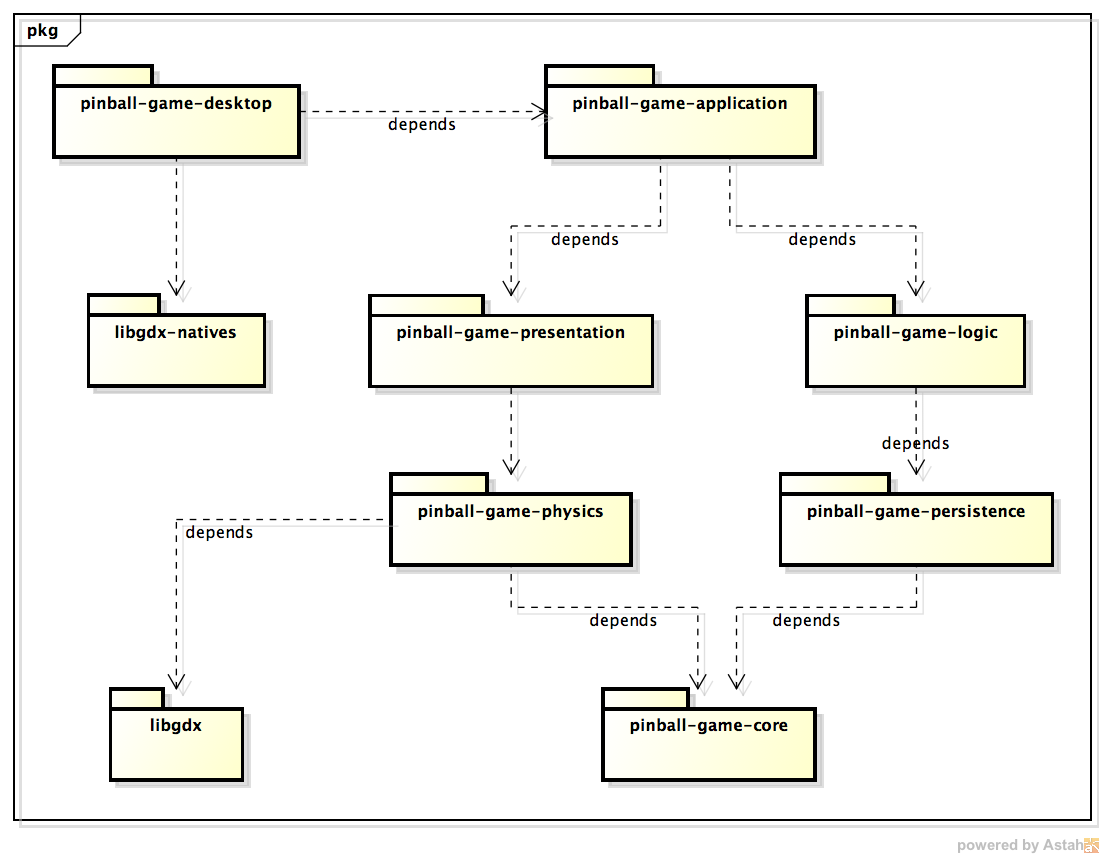
\includegraphics[width=15.5cm]{./img/package-overview.png}

\section{Persistence}

\subsection{Play field}
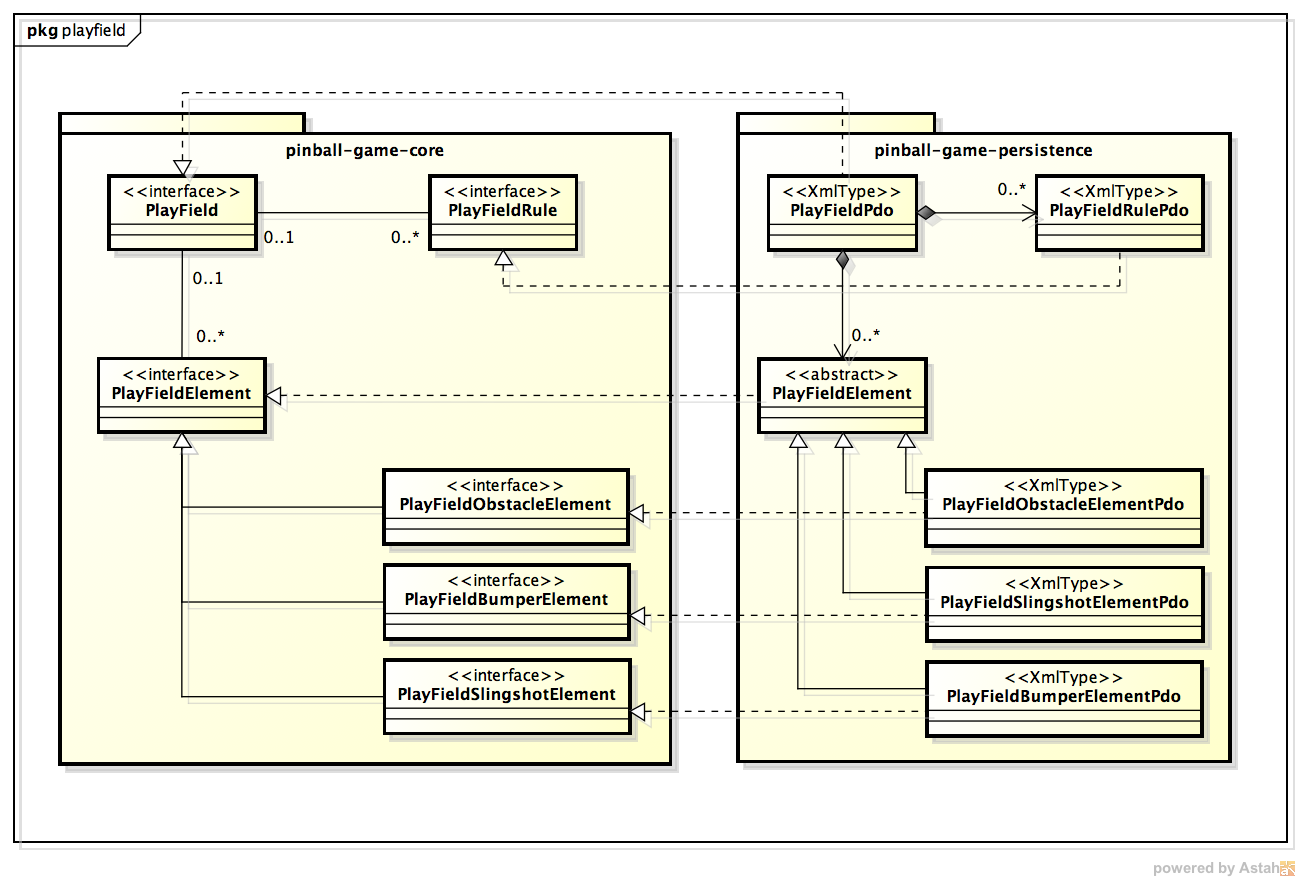
\includegraphics[width=15.5cm]{./img/persistence-playfield.png}

blah blah blah blah blah blah blah blah blah blah blah blah blah blah blah blah 
blah blah blah blah blah blah blah blah blah blah blah blah blah blah blah blah

\subsection{XML Schema}


\begin{lstlisting}[language=xml,label=lst:default_playfield,caption={schema for playfields.xml}]

<?xml version="1.0" encoding="UTF-8" standalone="yes"?>
<xs:schema version="1.0" targetNamespace="http://comet.m02.ch/pinball/playfield" xmlns:tns="http://comet.m02.ch/pinball/playfield" xmlns:xs="http://www.w3.org/2001/XMLSchema">

  <xs:element name="configuration" type="tns:configuration"/>

  <xs:complexType name="configuration">
    <xs:sequence>
      <xs:element name="playfields" form="qualified">
        <xs:complexType>
          <xs:sequence>
            <xs:element name="playfield" type="tns:playfield" form="qualified" maxOccurs="unbounded"/>
          </xs:sequence>
        </xs:complexType>
      </xs:element>
    </xs:sequence>
  </xs:complexType>

  <xs:complexType name="playfield">
    <xs:sequence>
      <xs:element name="name" type="xs:string" form="qualified"/>
      <xs:element name="elements" form="qualified">
        <xs:complexType>
          <xs:sequence>
            <xs:choice minOccurs="0" maxOccurs="unbounded">
              <xs:element name="bumper" type="tns:bumper" form="qualified"/>
              <xs:element name="slingshot" type="tns:slingshot" form="qualified"/>
              <xs:element name="obstacle" type="tns:obstacle" form="qualified"/>
            </xs:choice>
          </xs:sequence>
        </xs:complexType>
      </xs:element>
      <xs:element name="rules" form="qualified">
        <xs:complexType>
          <xs:sequence>
            <xs:element name="rule" type="tns:rule" form="qualified" maxOccurs="unbounded"/>
          </xs:sequence>
        </xs:complexType>
      </xs:element>
    </xs:sequence>
  </xs:complexType>

  <xs:complexType name="bumper">
    <xs:complexContent>
      <xs:extension base="tns:element">
        <xs:sequence>
          <xs:element name="radius" type="xs:float" form="qualified"/>
        </xs:sequence>
      </xs:extension>
    </xs:complexContent>
  </xs:complexType>

  <xs:complexType name="element" abstract="true">
    <xs:sequence>
      <xs:element name="id" type="xs:int" form="qualified"/>
      <xs:element name="position" type="tns:vector" form="qualified"/>
    </xs:sequence>
  </xs:complexType>

  <xs:complexType name="vector">
    <xs:sequence>
      <xs:element name="x" type="xs:float" form="qualified"/>
      <xs:element name="y" type="xs:float" form="qualified"/>
    </xs:sequence>
  </xs:complexType>

  <xs:complexType name="slingshot">
    <xs:complexContent>
      <xs:extension base="tns:element">
        <xs:sequence>
          <xs:element name="corner.a" type="tns:vector" form="qualified"/>
          <xs:element name="corner.b" type="tns:vector" form="qualified"/>
        </xs:sequence>
      </xs:extension>
    </xs:complexContent>
  </xs:complexType>

  <xs:complexType name="obstacle">
    <xs:complexContent>
      <xs:extension base="tns:element">
        <xs:sequence>
          <xs:element name="vertices" form="qualified">
            <xs:complexType>
              <xs:sequence>
                <xs:element name="vertice" type="tns:vector" form="qualified" maxOccurs="unbounded"/>
              </xs:sequence>
            </xs:complexType>
          </xs:element>
        </xs:sequence>
      </xs:extension>
    </xs:complexContent>
  </xs:complexType>

  <xs:complexType name="rule">
    <xs:sequence>
      <xs:element name="class" type="xs:string" form="qualified"/>
      <xs:element name="parameters" form="qualified">
        <xs:complexType>
          <xs:sequence>
            <xs:element name="parameter" type="xs:int" form="qualified" maxOccurs="unbounded"/>
          </xs:sequence>
        </xs:complexType>
      </xs:element>
    </xs:sequence>
  </xs:complexType>
</xs:schema>
\end{lstlisting}

\subsection{playfields.xml}
\begin{lstlisting}[language=xml,label=lst:default_playfield,caption={example of playfields.xml}]
<?xml version="1.0" encoding="UTF-8"?>
<configuration xmlns="http://comet.m02.ch/pinball/playfield" xmlns:xsi="http://www.w3.org/2001/XMLSchema-instance"
		xsi:schemaLocation="http://comet.m02.ch/pinball/playfield https://raw.github.com/boskoop/comet-pinball/master/schema/playfield.xsd">
	<playfields>
		<playfield>
			<name>default</name>
			<elements>
				<bumper>
					<id>1</id>
					<position>
						<x>0.25</x>
						<y>1.1</y>
					</position>
					<radius>0.03</radius>
				</bumper>
				<bumper>
					<id>2</id>
					<position>
						<x>0.45</x>
						<y>1.1</y>
					</position>
					<radius>0.03</radius>
				</bumper>
				<bumper>
					<id>3</id>
					<position>
						<x>0.35</x>
						<y>1.05</y>
					</position>
					<radius>0.03</radius>
				</bumper>
				<slingshot>
					<id>4</id>
					<position>
						<x>0.07</x>
						<y>0.355</y>
					</position>
					<corner.a>
						<x>0.12</x>
						<y>-0.09</y>
					</corner.a>
					<corner.b>
						<x>0.0</x>
						<y>0.1</y>
					</corner.b>
				</slingshot>
				<slingshot>
					<id>5</id>
					<position>
						<x>0.65</x>
						<y>0.355</y>
					</position>
					<corner.a>
						<x>0.0</x>
						<y>0.1</y>
					</corner.a>
					<corner.b>
						<x>-0.12</x>
						<y>-0.09</y>
					</corner.b>
				</slingshot>
				<obstacle>
					<id>6</id>
					<position>
						<x>0.65</x>
						<y>1.0</y>
					</position>
					<vertices>
						<vertice>
							<x>0.0</x>
							<y>0.0</y>
						</vertice>
						<vertice>
							<x>0.0</x>
							<y>0.15</y>
						</vertice>
						<vertice>
							<x>-0.12</x>
							<y>-0.09</y>
						</vertice>
					</vertices>
				</obstacle>
				<obstacle>
					<id>7</id>
					<position>
						<x>0.07</x>
						<y>1.0</y>
					</position>
					<vertices>
						<vertice>
							<x>0.0</x>
							<y>0.0</y>
						</vertice>
						<vertice>
							<x>0.12</x>
							<y>-0.09</y>
						</vertice>
						<vertice>
							<x>0.0</x>
							<y>0.15</y>
						</vertice>
					</vertices>
				</obstacle>
				<obstacle>
					<id>8</id>
					<position>
						<x>0.35</x>
						<y>0.5</y>
					</position>
					<vertices>
						<vertice>
							<x>0.08</x>
							<y>0.04</y>
						</vertice>
						<vertice>
							<x>-0.08</x>
							<y>0.04</y>
						</vertice>
						<vertice>
							<x>-0.00</x>
							<y>-0.04</y>
						</vertice>
					</vertices>
				</obstacle>
				<slingshot>
					<id>9</id>
					<position>
						<x>0.35</x>
						<y>0.54</y>
					</position>
					<corner.a>
						<x>0.0</x>
						<y>0.08</y>
					</corner.a>
					<corner.b>
						<x>-0.08</x>
						<y>0.00</y>
					</corner.b>
				</slingshot>
				<slingshot>
					<id>10</id>
					<position>
						<x>0.35</x>
						<y>0.54</y>
					</position>
					<corner.a>
						<x>0.08</x>
						<y>0.00</y>
					</corner.a>
					<corner.b>
						<x>0.0</x>
						<y>0.08</y>
					</corner.b>
				</slingshot>
			</elements>
			<rules>
				<rule>
                    <class>ch.m02.comet.pinball.logic.simulation.rule.basic.HitScoreRule</class>
                    <parameters>
                        <parameter>1</parameter>
                        <parameter>20</parameter>
                    </parameters>
				</rule>
				<rule>
                    <class>ch.m02.comet.pinball.logic.simulation.rule.basic.HitScoreRule</class>
                    <parameters>
                        <parameter>2</parameter>
                        <parameter>20</parameter>
                    </parameters>
				</rule>
				<rule>
                    <class>ch.m02.comet.pinball.logic.simulation.rule.basic.HitScoreRule</class>
                    <parameters>
                        <parameter>3</parameter>
                        <parameter>20</parameter>
                    </parameters>
				</rule>
				<rule>
                    <class>ch.m02.comet.pinball.logic.simulation.rule.basic.HitScoreRule</class>
                    <parameters>
                        <parameter>4</parameter>
                        <parameter>5</parameter>
                    </parameters>
				</rule>
				<rule>
                    <class>ch.m02.comet.pinball.logic.simulation.rule.basic.HitScoreRule</class>
                    <parameters>
                        <parameter>5</parameter>
                        <parameter>5</parameter>
                    </parameters>
				</rule>
			</rules>
		</playfield>
	</playfields>
</configuration>
\end{lstlisting}


\subsection{Simulation}

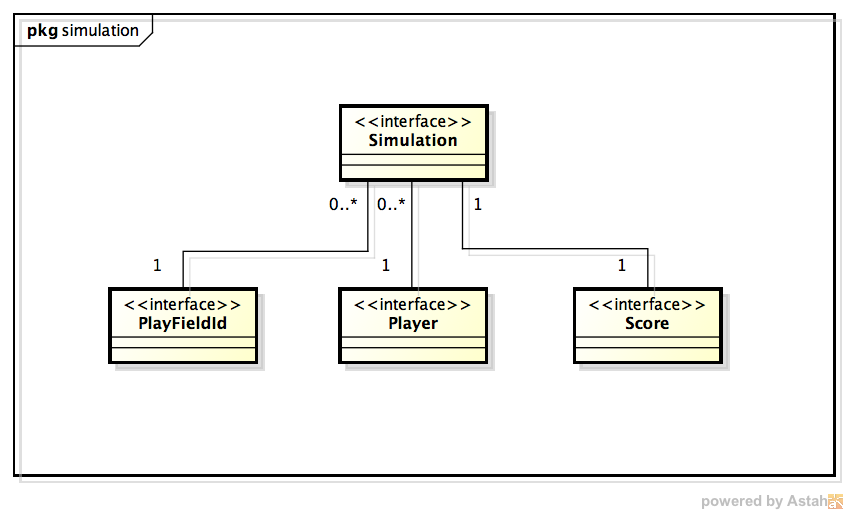
\includegraphics[width=15.5cm]{./img/persistence-simulation.png}

blah blah blah blah blah blah blah blah blah blah blah blah blah blah blah blah 
blah blah blah blah blah blah blah blah blah blah blah blah blah blah blah blah

\section{Dependency injection}
\subsection{Why dependency injection?}
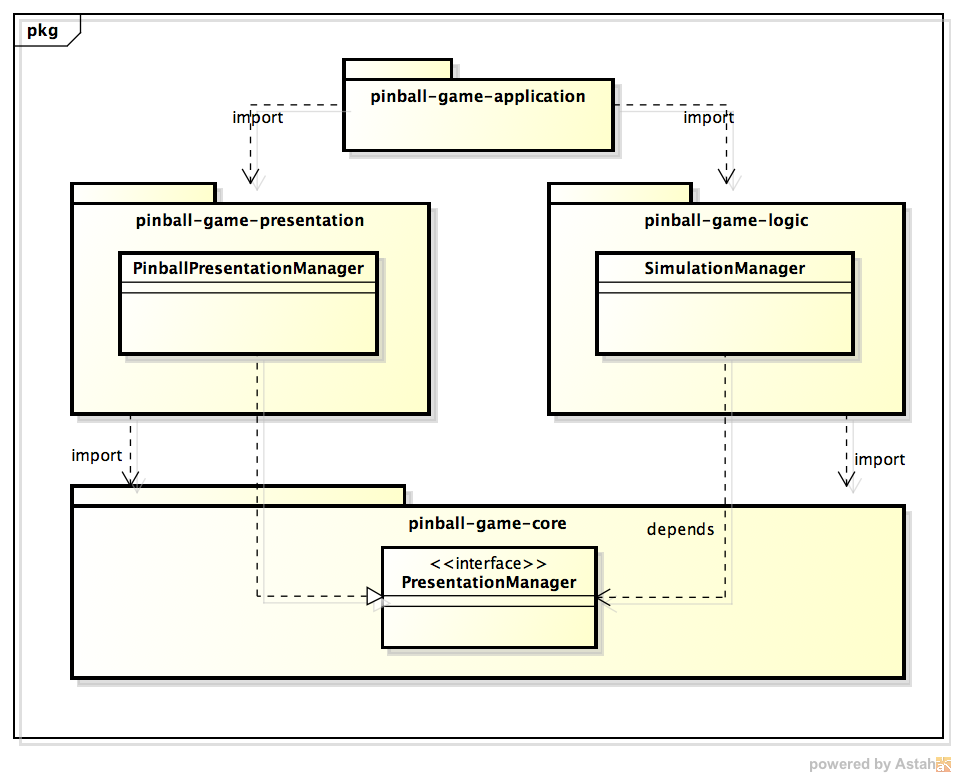
\includegraphics[width=15.5cm]{./img/dependency-injection1.png}

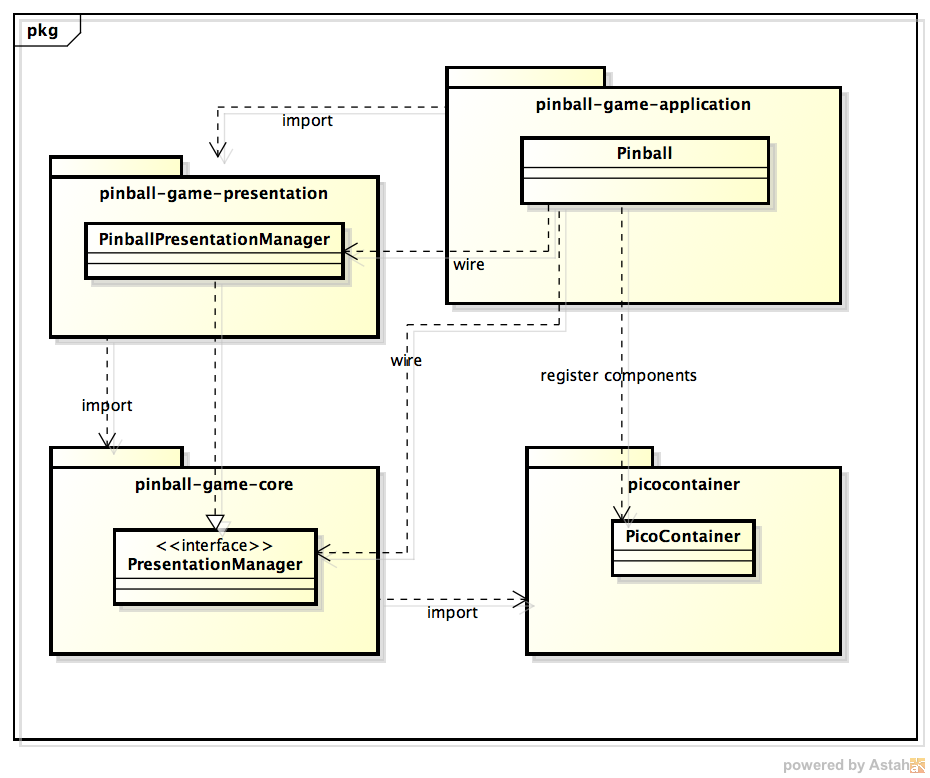
\includegraphics[width=15.5cm]{./img/dependency-injection2.png}

\subsection{Sequence diagram}
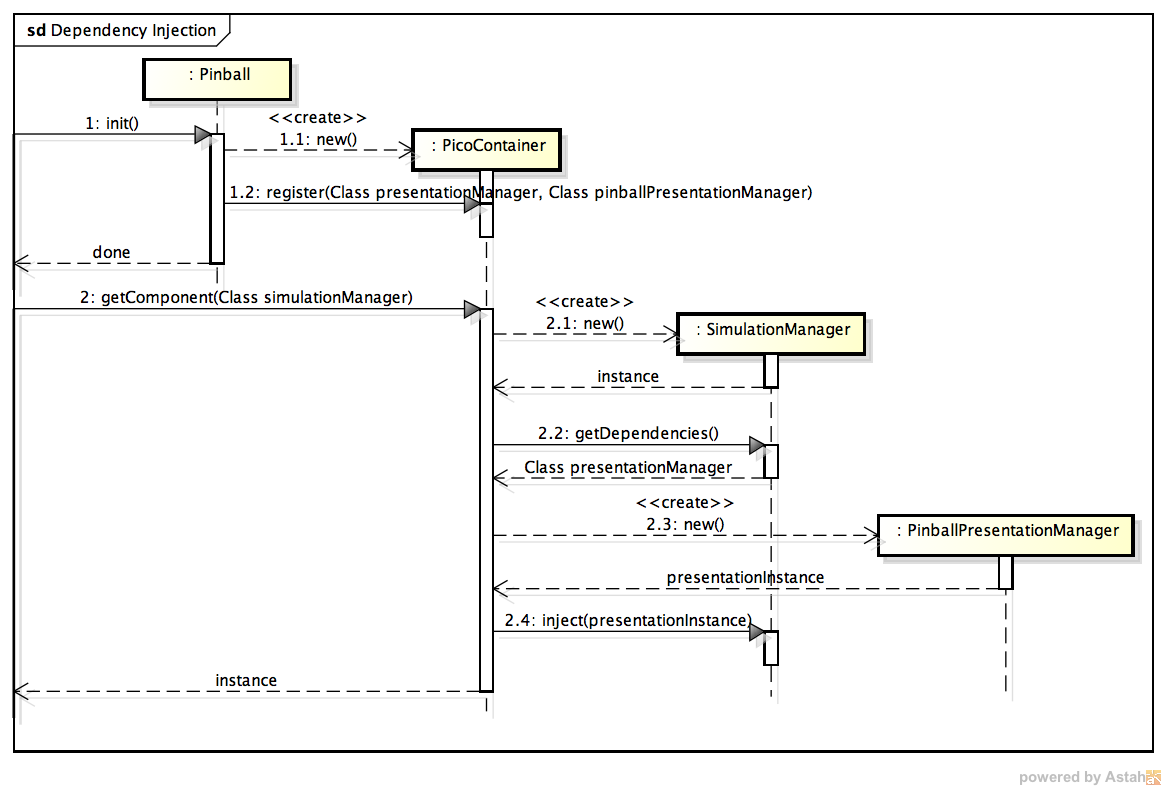
\includegraphics[width=15.5cm]{./img/dependency-injection-sd.png}

\section{Communication between modules}
\subsection{Command pattern}
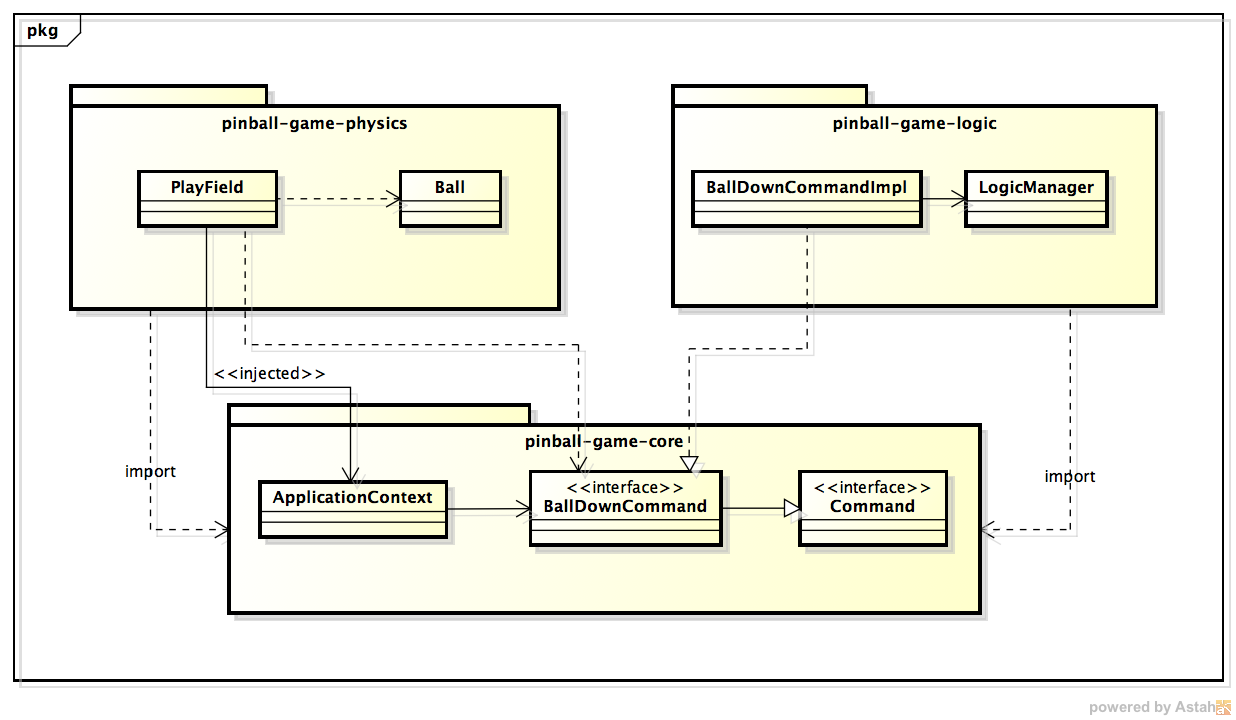
\includegraphics[width=15.5cm]{./img/command-pattern1.png}

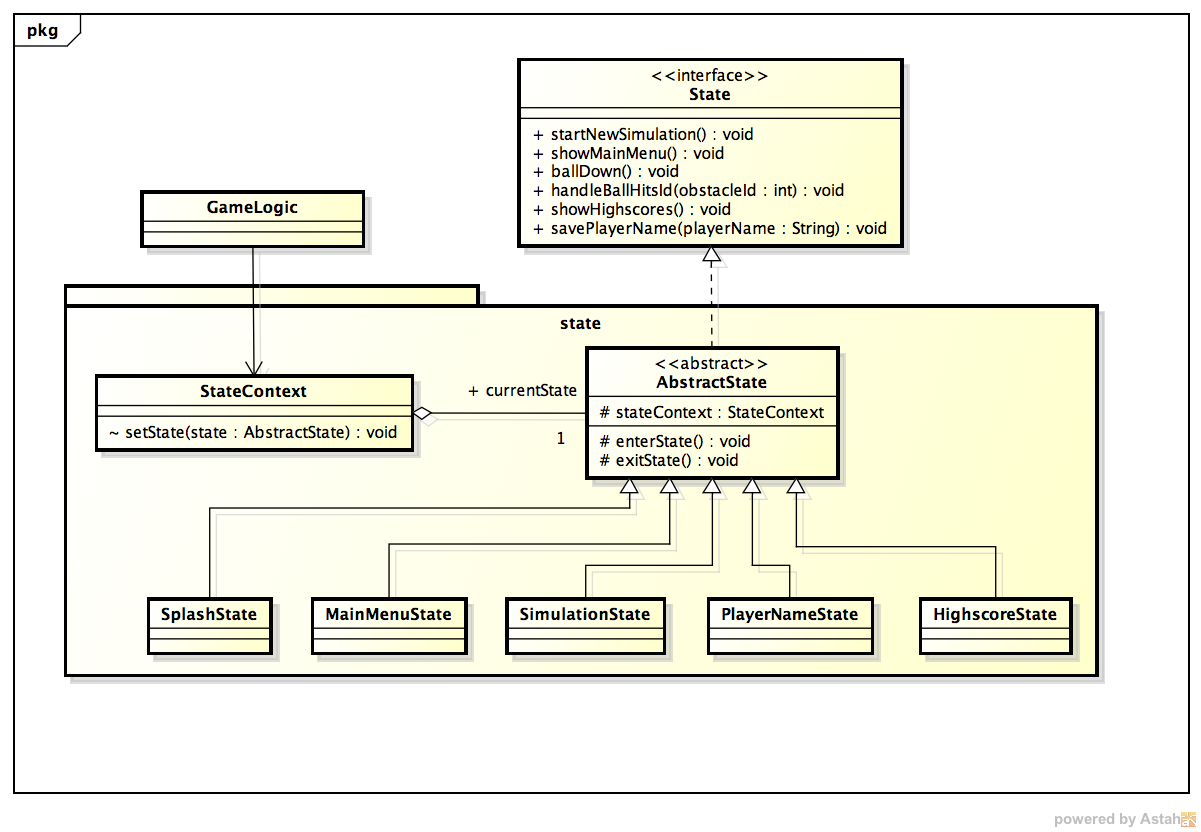
\includegraphics[width=15.5cm]{./img/command-pattern2.png}


\section{State machine}
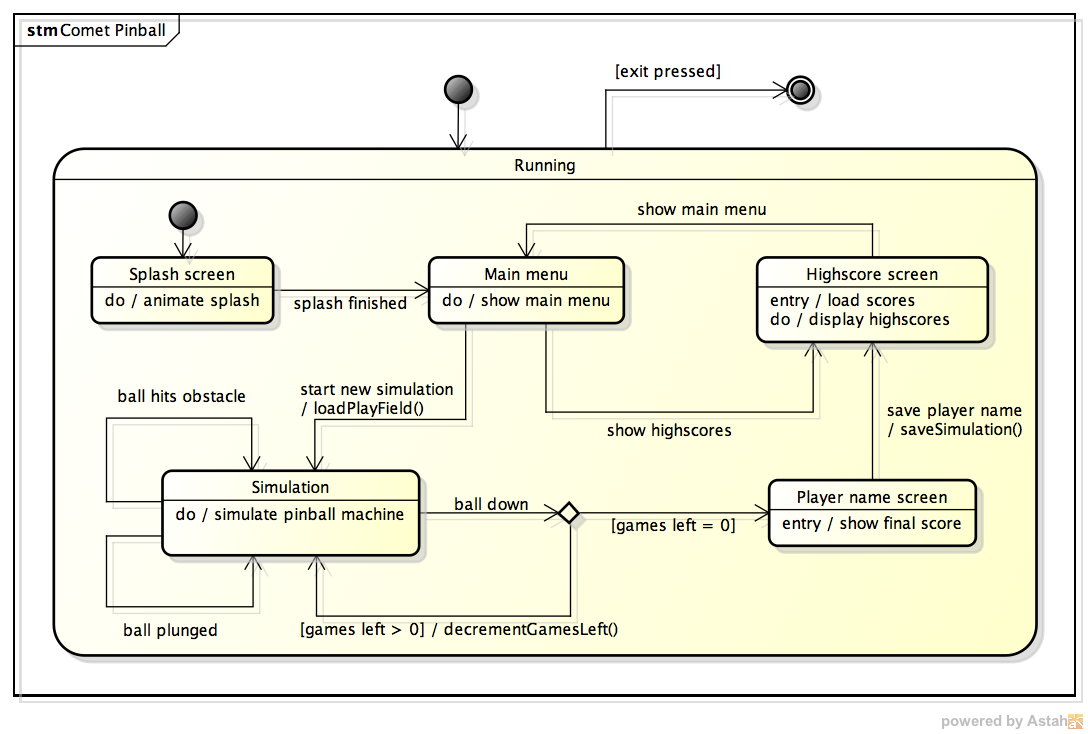
\includegraphics[width=15.5cm]{./img/state-machine.png}


\end{document}
